% Case description: Inscripta 
% deployment setup diagram
% \begin{figure*}[t]
% \centering
% 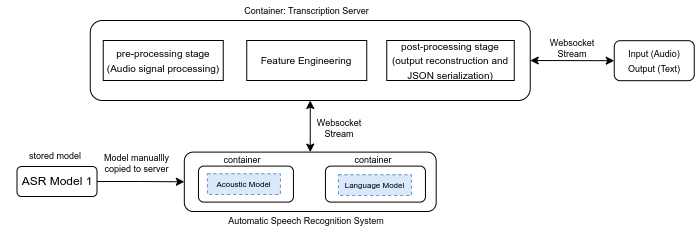
\includegraphics[width=0.8\textwidth]{images/case3_deployment_process_v2.png}
% \caption{Case 3 Inference Architecture}
% \label{fig: case3_deployment_process}
% \end{figure*}

% Case Description: Noice
% deployment setup diagram
\begin{figure*}[t]
\centering
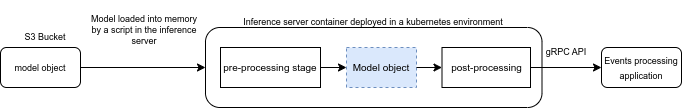
\includegraphics[width=0.8\textwidth]{images/case2_deployment_process_v2.png}
\caption{Case 2 Inference Architecture}
\label{fig: case2_deployment_process}
\end{figure*}

The ML system is an automated speech recognition system designed to transcribe speech data into text for medical and customer service applications. The two applications are based on two distinct models; a medical model trained on medical data and a model trained on business context data. These two types of models are deployed in two independent clusters. However, both systems process streaming speech data and produce transcribed text data. The primary difference lies in the model being deployed. The speech data is collected by a client and streamed to the backend server for transcription. Transcription results are sent to a web application or the client. The transcription service provides a real-time user experience; therefore, the application's performance after deployment is critical.

\textit{Pre-integration}: Trained models are stored in a cloud server and manually copied to the respective inference server with updated configuration files. A rigorous automated CI/CD pipeline ensures high-quality models are deployed, where models undergo testing, building, staging, and production stages. 

\textit{Quality assurance}: The testing phase involves performing local quick checks and unit tests, then building a docker image of the model. An end-to-end and integration test is conducted on the resulting image, and the docker image is deployed to a staging environment for re-testing. A version of the model is approved for deployment to the production environment after all tests have passed. 

\textit{Server environment}: The inference server is versioned, and each version instance contains a unique model version. The server is packaged as a docker image and deployed in a Kubernetes environment, ensuring the deployment can work across multiple vendors. The model in medical deployment is generally stable from a training perspective and serves various medical contexts. On the other hand, the customer service models tend to drift easily, and the deployment contains about 20 model variants. %In general, the deployment architecture is designed to work in multi-vendor settings, and the system comprises two deployment clusters: the medical and the customer service deployment.

\textit{Inference}: The inference pipeline contains similar components across the two deployment clusters (medical and customer service), making it easy to swap models, scale, and replicate the service. Replication supports multiple languages; each language can be scaled according to the number of users. The pipeline contains the following stages: i) a pre-processing step where audio data is converted into raw wave files with a fixed sampling rate, empty sections of the audio file are skipped, and feature extraction algorithms are applied, ii) the transformed data is sent to the ML server through a WebSocket connection, and ii) the inference is converted to JSON format for web applications to use. This pipeline runs in real-time, streaming data to the WebSocket server and presenting the results to the user. This inference architecture is shown in Figure~\ref{fig: case3_deployment_process}.

\textit{Monitoring}: The system is mainly monitored for latency and general availability. Real-time inference is essential for online deployment, and the system must also be highly available to its users. The models are monitored for drift based on customer feedback. In extreme cases where a customer experiences significant degradation in performance, a dedicated model can be provisioned for that customer based on updated training data or other configurations in the model.
